\documentclass[UTF-8]{ctexart}


\usepackage{url}
\usepackage{cite}
\usepackage[version=4]{mhchem}
\usepackage{graphicx}
\usepackage{subfigure}
\usepackage[a4paper,top=2cm,bottom=2cm,right=3cm,left=3cm,marginparwidth=1.75cm]{geometry}
\usepackage{amsmath}

\title{人机交互中的电磁学原理}
\author{闫皓铭 \\ 元培学院 2300017744}
\date{Autumn, 2024}


\begin{document}
\maketitle

\section{引言}
作为整合科学专业的学生,我一直试图在与生物学相关的多学科交叉的领域中,寻找一些和电磁学课程联系紧密的,有趣新颖的话题和对象,作为本次读书报告的主题。
最终决定阅读和“人机交互”相关的书籍,并把我的一些收获总结在这篇报告中。

人机交互在我们的日常生活中已经非常普遍了,这里所谓的“机”,以手机、平板等电子设备为典型代表。
而电子设备中,自然涉及到诸多电磁学知识作为其原理,与此同时,在不同应用场景中,展现出很大的灵活性、多样性与实用性。
而人机交互也离不开人的感官和感觉。交互方式通常涉及“视觉”、“听觉”和“触觉”。
为了实现更好的人机交互效果,相关电子设备的设计都基于人类的生物学特征和基本的生物学原理。

通过相关资料与书目的阅读,我对很多日常中习以为常的设备的工作原理有了更深刻的认识,
对电磁学理论的应用有了更丰富的认识,对生物学相关知识有了更生动的认识。
\section{视觉交互——屏幕} 
\subsection{屏幕显示技术:侧重非主动发光显示机理}

\subsection{屏幕触控技术}
我主要调查了解了三种触控技术:电阻式、电容式、压电式。
它们的技术原理各不相同,具备的功能与应用场景也有很大差别。
然而就电磁学原理的角度来看,它们主要运用了静电场和电介质的知识。
\subsubsection{电阻式触控:联系静电场与直流电路部分知识}


电阻式触控的基本原理是基于匀强电场,电势与位移成正比:
$$
E = -\nabla \varphi=\text{定值}   
$$
$$
\frac{\text{测量电势}}{\text{供电电压}}=\frac{\varphi_1}{\varphi_2-\varphi_1}=\frac{d_1}{d_2-d_1}=\frac{\text{测量位置}}{\text{屏幕宽度}}
$$
匀强电场是在上下两层电阻中形成的\cite{Touch},参考图\ref{电阻式触控原理}。
上下两侧电场相互正交,是为了测量$(x,y)$两个坐标。
上下两层的电场是交替形成的。工作机制是这样的:上层形成电场,下层进行测量;下层形成电场,上层进行测量;二者交替进行。
\begin{figure}
    \centering
    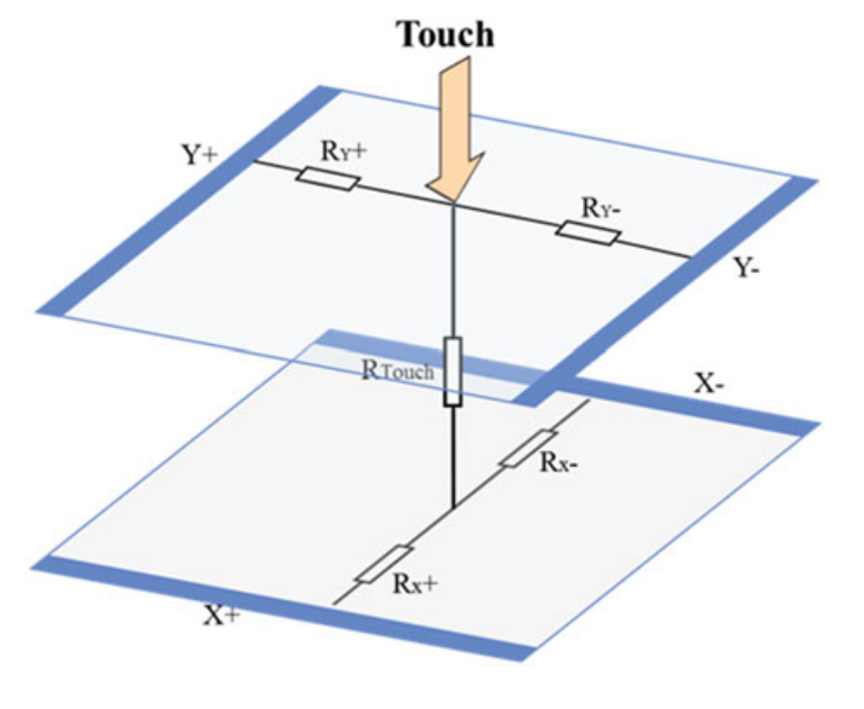
\includegraphics[width=0.5\linewidth]{../Figures/resistive.png}
    \caption{电阻式触控原理\cite{Touch}}
    \label{电阻式触控原理}
\end{figure}
从材料的角度看,上下两层导电层是\ce{In}与\ce{Sn}的氧化物,叫做(Indium Tin Oxide, ITO),具有透明的良好属性\cite{ITO}。
导电层之间用绝缘材料隔开,只有在用力按压触摸时,才相互接触,从而可以互相测量电势,进而探测位置。

这种电阻式的触控对于施力物体的电学性质没有要求。
这既是优点,也是缺点。
根据我的观察,咱们学校文史楼一些教室安装的屏幕就具有这种特点。
用塑料的签字笔,便可以实现对屏幕的触控,从而可以在屏幕上写字。
从而可以推断,该屏幕带概率时电阻式的触控屏。
但我们的手机显然不是这样的,因为从这个原理来看,电阻式的触控屏只能支持单点触控,不能实现多点触控。
此外,这会增加手机误触的风险。比如揣在兜里的手机可能会被意外触控。

\subsubsection{电容式触控:联系电容器部分知识}

\begin{figure}
    \centering
    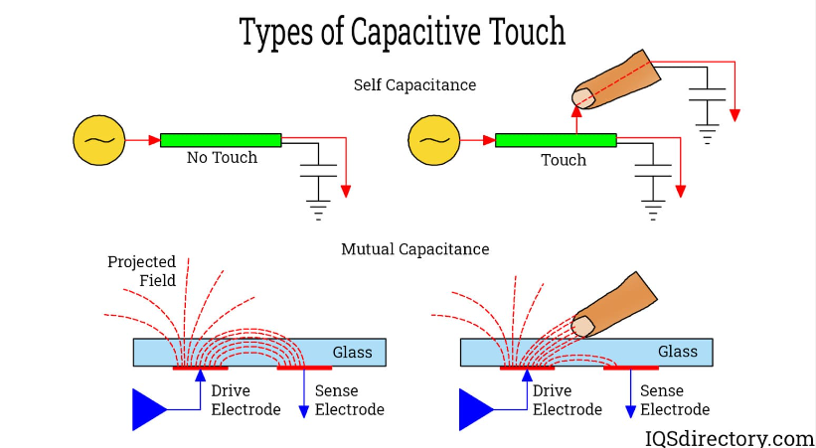
\includegraphics[width=0.7\linewidth]{../Figures/capacitive.png}
    \caption{电容式触控原理\cite{Capacitive}}
    \label{电容式触控原理}
\end{figure}

电容式触控种类繁多,我在这里分析两类。一类是所谓“自电容”类型,另一类是“互电容”类型。
它们的工作原理参考图\ref{电容式触控原理}。

首先可以明确的是,在这个模型中,人视作导体,并且接地。
手指与极板接近,则相当于增加了一个电容。
两种机制的最大区别在于,“自电容”测量的是驱动电极与大地之间的电容,而“互电容”测量的是驱动电极与接收电极之间的电容。

在“自电容”机制中,手指(此处视作导体)的接近,相当于给原本存在的寄生电容并联了一个电容。
从而总电容(待测电容)\textbf{增大}。

而在“互电容”中,驱动电极与接收电极之间形成的电容器是开放式的,这一点与常见电容器不同。
手指,作为导体的靠近,使得电场线更多地指向手指。
换言之,手指改变了原本的电场分布(这个电场被称为投射电场)。
从图\ref{电容式触控原理}可见,这相当于减少了有效正对面积,从而手指的靠近使被测电容值(驱动电极与接收电极之间,而非总电容)\text{减小}\cite{Capacitive}。

电容的测量涉及反复充放电的过程。而对于位置的确定,经过了对全平面多个测量子区域的反复扫描。
这种扫描的时延不为我们用户所感知,但无疑是工程师考虑的重点。
“互电容”因为机制复杂,所以扫描周期更长,时延更大。

一个有趣的现象是,“自电容”机制支持一点触控或两点放缩(可以双指放大或缩小页面),却也仅支持放缩操作。
“互电容”则可以支持更多点的触控。

“互电容”支持多点触控相对好理解,因为它将全平面划分为多个子区域,并且彼此独立(相邻两极板间的电容),测量互不干扰。

“自电容”则不然。由于它测量的是对地的总电容,从而各个子区域并不独立。
具体结构可以参考图\ref{“自电容”机制中的邻顶点与对顶点}中的示意。
具体来讲,各列与各列独立,但是一列之内不可区分。各行与各行独立,但是一行之内不可区分。
当仅有一个触摸点的时候,取一行与一列的交点即可唯一确定位置。
但是有两个触摸点的时候,两行两列形成四个交点,究竟是哪两个点?结果并不能唯一确定。
有趣的是,这并不影响双指放缩的操作,因为这个操作只关心双指之间的距离,与具体位置无关。
从而这一功能是可以实现的。
\begin{figure}
    \centering
    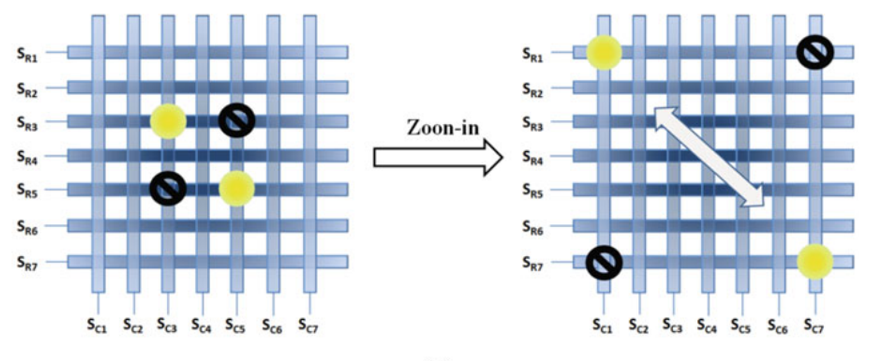
\includegraphics[width=0.9\linewidth]{../Figures/self.png}
    \caption{“自电容”机制中的邻顶点与对顶点不可分辨性与双指放缩操作的可行性\cite{Touch}}
    \label{“自电容”机制中的邻顶点与对顶点}
\end{figure}


电容式较电阻式有明显优势,更多地被精密的屏幕所采用。
但也应注意到,电容式触控只关心电学性质,而不能够探测施加的力的大小,而电阻式可以。
此外,这也解释了为什么我们冬天戴手套很多操作手机。因为手套的绝缘面料阻断了这一感应机制。
\subsubsection{压电式触控:联系电介质部分知识}
压电现象指的是,施加压力后电介质表面产生电荷。压电现象的逆效应也被实验证实。
也就是说,压电现象的正逆效应是电信号与力学信号转化的又一座桥梁(电磁感应或许是最经典的桥梁)。

与课内学习的电介质极化机制不同,压电效应的电介质极化来自于外界施加压力而非外电场。
这种神奇的现象,本质上源自于分子结构缺乏中心对称性,参考图\ref{压电效应的分子机制 }。
\begin{figure}
    \centering
    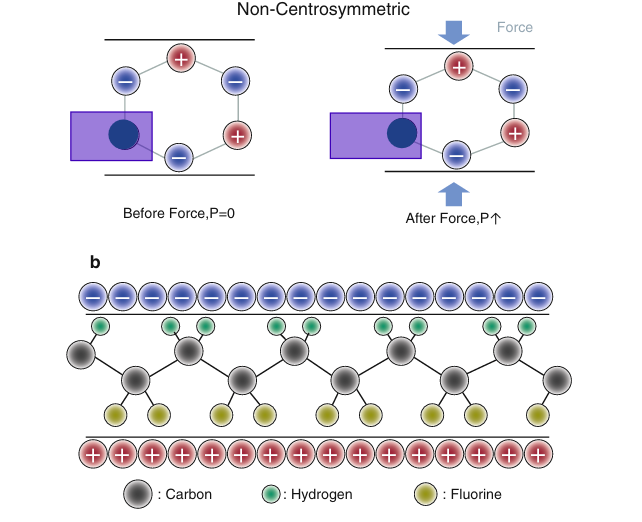
\includegraphics[width=0.7\linewidth]{../Figures/piezoelectric.png}
    \caption{压电效应的分子机制(poly(vinylidene fluoride), PVDF)\cite{Touch}}
    \label{压电效应的分子机制 }
\end{figure}
电极化强度矢量由应力决定:
$$
P=\tilde{d}\sigma\quad,\sigma\text{表示应力}
$$
电极化强度矢量决定了表面电荷密度:
$$
\sigma_{e}=\vec{P}\cdot \vec{n}
$$
电压由电荷产生:
$$
U=\frac{Q}{C}=\frac{\sigma_{e}S}{\frac{\varepsilon _0 \varepsilon _r S}{t}}=\frac{\tilde{d}\sigma S}{\frac{\varepsilon _0 \varepsilon _r S}{t}}=\frac{t\tilde{d} }{\varepsilon _0 \varepsilon _r}\cdot{\sigma}
$$
而归根结底,电压是由应力决定的。
\begin{figure}
    \centering
    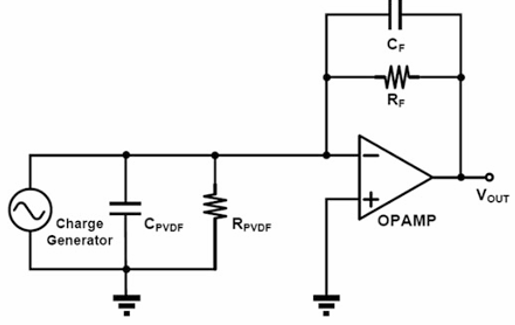
\includegraphics[width=0.6\linewidth]{../Figures/opamp.png}
    \caption{运算放大器构成的积分器实现电荷增益\cite{Touch}}
    \label{运放}
\end{figure}


而压电效应产生的电荷与电压都是很小的。实际应用中,采用了运算放大器进行信号增益。
具体来讲,使用了一个由运算放大器构成的积分器\cite{circuit},实现对电压的积分,也就是对电荷的测量,如图\ref{运放}。
为了达到更好的电荷增益效果,应该选用较小的电容器$C_F$。
$$
V_{out}=-\frac{1}{R_FC_F}\int V_{in} dt=-\frac{Q}{R_FC_F}
$$
而由于触控是一个低频信号,所以应采用较大的电阻器$R_F$,与电容器一起构成一个低通滤波器。
$$
f_{\text{cut off}}=\frac{1}{2\pi R_FC_F}
$$

压电效应技术并不十分成熟,还在广泛的研究之中。
但是,它和电容式的触控联合使用,可以同时实现对力学量的测量,以及多点触控等良好的控制效果。
此外,由于压电效应本身并不依赖于供电电源,这使得它的功耗较低。
除了显示屏幕,这种新技术也被用于可穿戴电子设备,进一步丰富了人机交互的途径。


\section{触觉交互}
\subsection{触摸行为的生物学特质}
准确刻画触摸行为的生物学特质至关重要,比如在打电话的时候要排除掉面部和手机屏幕接触引发的误触干扰。
要准确的计算出触摸中心,而且计算方法应该对于成人和小孩都适用。
这个过程中,除了要关注手指的几何参数(长宽以及曲率)还要关注电学参数(电导),这一点对于电阻式触控没有影响,但对电容式触控影响显著。

此外,在书写、绘画等过程中,用力的大小通常转化为线条的粗细。
那么这就要求对人用力的相对值,有一个较为准确的测量方法。

与此同时,工程上还要考虑到噪音处理的问题。
鉴于人的触摸频率是比较低的,在10HZ一下,所以实际电路中,涉及许多低通滤波器来过滤噪音。

\subsection{振动的产生机制:联系电磁感应部分知识}
% Figure








% List
\begin{itemize}
    \item item 1
    \item item 2
\end{itemize}


\bibliographystyle{plain}
\bibliography{references}
\end{document}